\chapter{总体概述}

本节描述影响产品和产品需求的一般因素。由以下4个部分构成。 有一点需说明的是本节不描述具体的需求,只是使那些将要描述的具体需求更易于理解。
\section{软件概述}
\subsection{项目介绍}
应用商店的开发与时俱进,现在出现的PC端与手机端应用商店出现了严重的割裂,
而且应用的质量得不到保证、用户的反馈得不到及时的回应、开发者的合理权益得不到保障、
用户需要专门花时间去找应用等等问题层出不穷。

现在出现的应用商店无法解决这样问题,这也是本项目出现的主要原因,
即构建一个面向未来的、可拓展的、友好的应用商店系统。
以达到全面替代当前的各种应用商店的目的。


\subsection{产品环境介绍}

本项目构成一个独立的体系而且完全自我包含。

\section{软件功能}
为了便于设计和理解,将软件的功能分为三个组块,即开发者端、服务器端、用户端。


下面详细介绍。

\subsection{开发者端}
针对开发者,我们需要设定开发者是普通的应用程序开发人员甚至是非专业的,为了激发开发的参与,
本系统需要简化应用开发的门槛,因而开发者端需要尽可能简化。
\begin{itemize}
\item 应用管理

	\begin{itemize}
	\item 应⽤上传
	\item 应用更新
	\item 应用删除
	\end{itemize}
\item 信息反馈
	\begin{itemize}
	\item
	应⽤信息查询与管理
	\begin{itemize}
		\item 下载量
		\item 评论
		\item 回复
	\end{itemize}
	\item 收⼊查询与管理
	\begin{itemize}
		\item 提现
		\item 转账
	\end{itemize}
	\end{itemize}

\item \color{red}{应用开发}
	\begin{itemize}
		\item \color{red}{代码编辑}
		\item \color{red}{代码编译与运行}
		\item \color{red}{debug功能}
	\end{itemize}
\end{itemize}
	

\subsection{服务器端}
服务器端是一个增加了某些特殊功能的数据库,需要存储开发者、应用、用户的信息,以及相关的触发操作,
下面的列表详细地说明了其功能。

\begin{itemize}
\item 开发者管理系统
	\begin{itemize}
	\item 开发者信息维护
		\begin{itemize}
		\item 注册与注销
		\item 个人基本信息
		\item 开发的应用
		\end{itemize}
	\item 反馈内容
		\begin{itemize}
			\item 收入查询
			\item 收入提现
			\item 应用评分与评论
		\end{itemize}
	\end{itemize}
\item 应用管理系统
	\begin{itemize}
	\item 应用信息管理
		\begin{itemize}
		\item 基本信息
		\item 下载量
		\item 评价
		\item 评分
		\end{itemize}
	\item 应用上传、更新、删除、下载管理
		\begin{itemize}
			\item 应⽤审核
			\item 应⽤排名
			\item 应⽤推荐
		\end{itemize}
	\end{itemize}
\item ⽤户管理系统
	\begin{itemize}
	\item 用户信息维护
	\begin{itemize}
		\item 注册与注销
		\item 个人基本信息
		\item 下载/购买的应用
	\end{itemize}
	\end{itemize}
\item 第三方管理系统
	\begin{itemize}
	\item ⼴告投放管理
	\item 第三方资助管理
	\item 第三方监督管理
	\end{itemize}
\item \color{red}{应用开发管理系统}
\color{red}{
	\begin{itemize}
		\item 在线开发
		\item 在线预览
	\end{itemize}
}
\end{itemize}
	
\subsection{客户端}
\begin{itemize}
\item 应用管理
	\begin{itemize}
	\item 应⽤查询
	\item 应⽤购买
	\item 应⽤安装
	\item 应⽤更新
	\item 应用删除
	\end{itemize}
\item 信息反馈
	\begin{itemize}
	\item 应用评价
	\begin{itemize}
		\item 评分
		\item 评论
	\end{itemize}
	\end{itemize}
	\color{red}{
		\item 应用个性化
		\begin{itemize}
			\item 个性化配置
			\item 预览
		\end{itemize}	
		}
\end{itemize}

\subsection{需求关系}

\begin{figure}[ht]
	\centering
	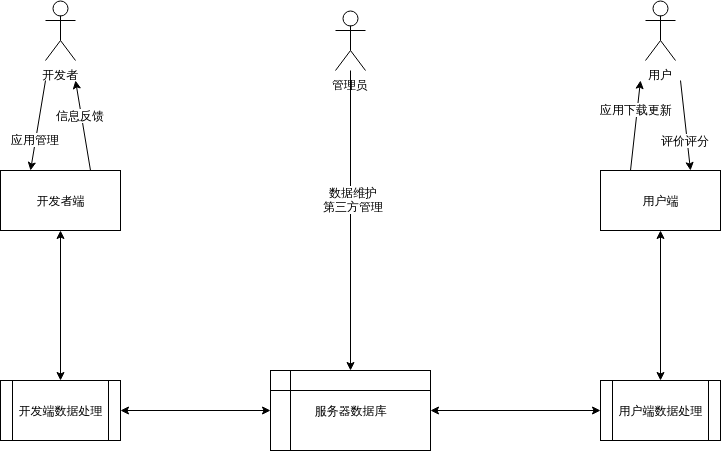
\includegraphics[width=10cm]{top_diagram.png}
	\caption{高层数据流图} \label{fig:top_diagram}
\end{figure}

下面的高层数据流图\ref{fig:top_diagram}简明扼要地说明了三个不同端之间的关系。


\section{用户特征}
开发者应该具有基本的开发能力,任何语言均可,本系统提供不同语言体系的打包与封装。

系统管理员应该具有基本的数据库维护能力。第三方的监督与广告投放应该交由管理员处理。

用户不假设具有任何的专业背景,要求是任何人均可以作为用户来使用本软件系统。


\section{假设和依赖关系}
本项目仅做最基本的假设,依赖于浏览器、网络协议、数据库以及具体的终端设备操作系统。

本项目尽可能面向未来,因而主要使用浏览器作为终端用户的交互设备,所以浏览器协议以及网络协议的改变
会对本项目造成影响。同时,鉴于部分用户的习惯依赖性,也需要提供相应的应用终端。
这一点需要考虑到不同PC或者手机的操作系统的架构。


